\chapter{solutions/magnetostatics}
\begin{abox}
	Practice set 1 solutions/magnetostatics
	\end{abox}
\begin{enumerate}
\begin{minipage}{\textwidth}
	\item The magnetic field at a distance $R$ from a long straight wire carrying a steady current $I$ is proportional to
	\exyear{NET 2012}
\end{minipage}
\begin{tasks}(2)
	\task[\textbf{A.}] $I R$
	\task[\textbf{B.}] $I / R^{2}$
	\task[\textbf{C.}]$I^{2} / R^{2}$
	\task[\textbf{D.}]$I / R$
\end{tasks}
\begin{answer}
	The correct option is \textbf{(d)}	
\end{answer}
\begin{minipage}{\textwidth}
	\item The vector potential $\vec{A}$ due to a magnetic moment $\vec{m}$ at a point $\vec{r}$ is given by $\vec{A}=\frac{\vec{m} \times \vec{r}}{r^{3}}$.
	If $\vec{m}$ is directed along the positive $z$-axis, the $x$ - component of the magnetic field, at the point $\vec{r}$, is
	\exyear{NET 2011}
\end{minipage}
\begin{tasks}(2)
	\task[\textbf{A.}] $\frac{3 m y z}{r^{5}}$
	\task[\textbf{B.}] $-\frac{3 m x y}{r^{5}}$
	\task[\textbf{C.}]$\frac{3 m x z}{r^{5}}$
	\task[\textbf{D.}]$\frac{3 m\left(z^{2}-x y\right)}{r^{5}}$
\end{tasks}
\begin{answer}
	\begin{align*}
	\vec{m}&=m \hat{z}\\
	 \text { and }\\
	 \vec{B}&=\vec{\nabla} \times \vec{A}=\frac{m}{r^{3}}(2 \cos \theta \hat{r}+\sin \theta \hat{\theta})=\frac{1}{r^{3}}[3(\vec{m} \cdot \hat{r}) \hat{r}-\vec{m}] \\
 \vec{B}&=\frac{1}{r^{3}}\left[3 m \hat{z} \cdot\left(\frac{x \hat{x}+y \hat{y}+z \hat{z}}{r}\right) \frac{\vec{r}}{r}-m \hat{z}\right] \\
   B_{x}&=\frac{3 m x z}{r^{5}}
	\end{align*}
\end{answer}
\begin{minipage}{\textwidth}
	\item An infinite solenoid with its axis of symmetry along the $z$-direction carries a steady current $I$.
	The vector potential $\vec{A}$ at a distance $R$ from the axis
	\exyear{NET 2012}
	\begin{figure}[H]
		\centering
		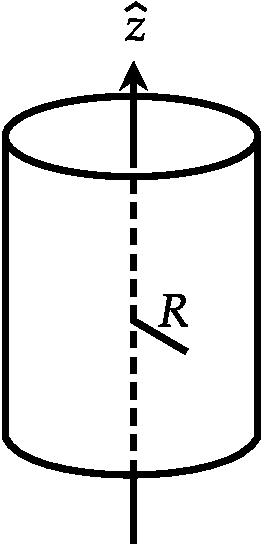
\includegraphics[height=4cm,width=3cm]{NET1}
	\end{figure}
\end{minipage}
\begin{tasks}(1)
	\task[\textbf{A.}]is constant inside and varies as $R$ outside the solenoid
	\task[\textbf{B.}] varies as $R$ inside and is constant outside the solenoid
	\task[\textbf{C.}]varies as $\frac{1}{R}$ inside and as $R$ outside the solenoid
	\task[\textbf{D.}]varies as $R$ inside and as $\frac{1}{R}$ outside the solenoid
\end{tasks}
\begin{answer}
	The correct option is \textbf{(d)}
\end{answer}
\begin{minipage}{\textwidth}
	\item The force between two long and parallel wires carrying currents $I_{1}$ and $I_{2}$ and separated by a distance $D$ is proportional to
	\exyear{NET 2013}
\end{minipage}
\begin{tasks}(2)
	\task[\textbf{A.}] $I_{1} I_{2} / D$
	\task[\textbf{B.}]$\left(I_{1}+I_{2}\right) / D$
	\task[\textbf{C.}]$\left(I_{1} I_{2} / D\right)^{2}$
	\task[\textbf{D.}]$I_{1} I_{2} / D^{2}$
\end{tasks}
\begin{answer}
	The correct option is \textbf{(a)}	
\end{answer}
\begin{minipage}{\textwidth}
	\item A time-dependent current $\vec{I}(t)=K t \hat{z}$ (where $K$ is a constant) is switched on at $t=0$ in an infinite current-carrying wire. The magnetic vector potential at a perpendicular distance $a$ from the wire is given (for time $t>a / c$ ) by
	\exyear{NET 2014}
\end{minipage}
\begin{tasks}(1)
	\task[\textbf{A.}] $\hat{z} \frac{\mu_{0} K}{4 \pi c} \int_{-\sqrt{c^{2} t^{2}-a^{2}}}^{\sqrt{c^{2} t^{2}-a^{2}}} d z \frac{c t-\sqrt{a^{2}+z^{2}}}{\left(a^{2}+z^{2}\right)^{1 / 2}}$
	\task[\textbf{B.}] $\hat{z} \frac{\mu_{0} K}{4 \pi} \int_{-c t}^{c t} d z \frac{t}{\left(a^{2}+z^{2}\right)^{1 / 2}}$
	\task[\textbf{C.}] $\hat{z} \frac{\mu_{0} K}{4 \pi c} \int_{-c t}^{c t} d z \frac{c t-\sqrt{a^{2}+z^{2}}}{\left(a^{2}+z^{2}\right)^{1 / 2}}$
	\task[\textbf{D.}] $\hat{z} \frac{\mu_{0} K}{4 \pi} \int_{-\sqrt{c^{2} t^{2}-a^{2}}}^{\sqrt{c^{2} t^{2}-a^{2}}} d z \frac{t}{\left(a^{2}+z^{2}\right)^{1 / 2}}$
\end{tasks}
\begin{answer}
	\begin{figure}[H]
		\centering
		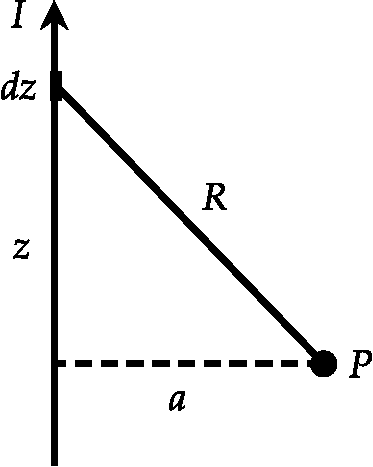
\includegraphics[height=4cm,width=5cm]{diagram-20211011(26)-crop}
	\end{figure}
	 \begin{align*}
	\vec{A} &=\hat{z} \frac{\mu_{0}}{4 \pi} \int_{-\infty}^{\infty} \frac{I\left(t_{r}\right)}{R} d z=\hat{z} \frac{\mu_{0}}{4 \pi} \int_{-\infty}^{\infty} \frac{K(t-R / c)}{R} d z \\
	\Rightarrow \vec{A} &=\hat{z} \frac{\mu_{0} K}{4 \pi c} \int_{-\sqrt{c^{2} t^{2}-a^{2}}}^{\sqrt{c^{2} t^{2}-a^{2}}} d z \frac{c t-\sqrt{a^{2}+z^{2}}}{\left(a^{2}+z^{2}\right)^{1 / 2}}
	\end{align*}
\end{answer}
\begin{minipage}{\textwidth}
	\item A charged particle moves in a helical path under the influence of a constant magnetic field. The initial velocity is such that the component along the magnetic field is twice the component in the plane normal to the magnetic field.
	The ratio $\ell / R$ of the pitch $\ell$ to the radius $R$ of the helical path is
	\exyear{NET 2014}
\end{minipage}
\begin{tasks}(2)
	\task[\textbf{A.}] $\pi / 2$
	\task[\textbf{B.}]$4 \pi$
	\task[\textbf{C.}]$2 \pi$
	\task[\textbf{D.}]$\pi$
\end{tasks}
\begin{answer}
	$v_{\|}=2 v_{\perp}$\\
	Pitch of the helix $l=v_{\|} T=v_{\|} \frac{2 \pi R}{v_{\perp}}=2 v_{\perp} \frac{2 \pi R}{v_{\perp}}=4 \pi R \Rightarrow \frac{l}{R}=4 \pi$
\end{answer}
\begin{minipage}{\textwidth}
	\item A proton moves with a speed of $300 \mathrm{~m} / \mathrm{s}$ in a circular orbit in the $x y$-plan in a magnetic field 1 tesla along the positive $z$-direction. When an electric field of $1 \mathrm{~V} / \mathrm{m}$ is applied along the positive $y$-direction, the center of the circular orbit
	\exyear{NET 2014}
\end{minipage}
\begin{tasks}(1)
	\task[\textbf{A.}] remains stationary
	\task[\textbf{B.}]moves at $1 \mathrm{~m} / \mathrm{s}$ along the negative $x$-direction
	\task[\textbf{C.}]moves at $1 \mathrm{~m} / \mathrm{s}$ along the positive $z$ - direction
	\task[\textbf{D.}] moves at $1 \mathrm{~m} / \mathrm{s}$ along the positive $x$ - direction
\end{tasks}
\begin{answer}
	Change particle will deflect in $+x$-direction with $v=\frac{E}{B}=\frac{1}{1}=1 \mathrm{~m} / \mathrm{s} .$\\
	The correct option is \textbf{(d)}	
\end{answer}
\begin{minipage}{\textwidth}
	\item Given a uniform magnetic field $B=B_{0} \hat{k}$ (where $B_{0}$ is a constant), a possible choice for the magnetic vector potential $A$ is
	\exyear{NET 2015}
\end{minipage}
\begin{tasks}(2)
	\task[\textbf{A.}] $B_{0} y \hat{i}$
	\task[\textbf{B.}] $-B_{0} y \hat{i}$
	\task[\textbf{C.}] $B_{0}(x \hat{j}+y \hat{i})$
	\task[\textbf{D.}]$B_{0}(x \hat{i}+y \hat{j})$
\end{tasks}
\begin{answer}
	(a) $\vec{\nabla} \times \vec{A}=-B_{0} \hat{k}$\\
	(b) $\vec{\nabla} \times \vec{A}=B_{0} \hat{k}$\\
	(c) $\vec{\nabla} \times \vec{A}=0$\\
	(d) $\vec{\nabla} \times \vec{A}=0$\\
	The correct option is \textbf{(b)}	
\end{answer}
\begin{minipage}{\textwidth}
	\item A small magnetic needle is kept at $(0,0)$ with its moment along the $x$-axis. Another small magnetic needle is at the point $(1,1)$ and is free to rotate in the $x y$ - plane. In equilibrium the angle $\theta$ between their magnetic moments is such that
	\exyear{NET 2015}
\end{minipage}
\begin{tasks}(2)
	\task[\textbf{A.}] $\tan \theta=\frac{1}{3}$
	\task[\textbf{B.}]$\tan \theta=0$
	\task[\textbf{C.}]$\tan \theta=3$
	\task[\textbf{D.}]$\tan \theta=1$
\end{tasks}
\begin{answer}
	\begin{figure}[H]
		\centering
		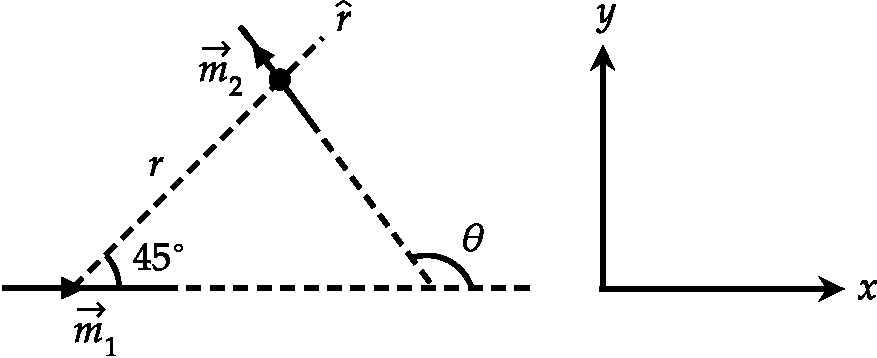
\includegraphics[height=4cm,width=6cm]{diagram-20211011(38)-crop}
	\end{figure}
	\begin{align*}
	&U=\frac{\mu_{0}}{4 \pi r^{3}}\left[\vec{m}_{1} \cdot \vec{m}_{2}-3\left(\vec{m}_{1} \cdot \hat{r}\right)\left(\vec{m}_{2} \cdot \hat{r}\right)\right]\\
	&U=\frac{\mu_{0} m_{1} m_{2}}{4 \pi r^{3}}\left[\cos \theta-3 \cos 45^{0} \cos \left(\theta-45^{0}\right)\right]
	\intertext{For stable position energy is minimum i.e.}
	&\frac{\partial U}{\partial \theta}=0 \Rightarrow \frac{\mu_{0} m_{1} m_{2}}{4 \pi r^{3}}\left[-\sin \theta+\frac{3}{\sqrt{2}} \sin \left(\theta-45^{\circ}\right)\right]=0 \\
	&\Rightarrow \sin \theta=\frac{3}{\sqrt{2}}\left(\frac{\sin \theta}{\sqrt{2}}-\frac{\cos \theta}{\sqrt{2}}\right) \Rightarrow \tan \theta=3
	\end{align*}
	The correct option \textbf{(c)}	
\end{answer}
\begin{minipage}{\textwidth}
	\item A dipole of moment $\vec{p}$, oscillating at frequency $\omega$, radiates spherical waves. The vector potential at large distance is\\
	$$\vec{A}(\vec{r})=\frac{\mu_{0}}{4 \pi} i \omega \frac{e^{i k r}}{r} \vec{p}$$	
	$\text { To order }\left(\frac{1}{r}\right) \text { the magnetic field } \vec{B} \text { at a point } \vec{r}=r \hat{n} \text { is }$
	\exyear{NET 2015}
\end{minipage}
\begin{tasks}(2)
	\task[\textbf{A.}] $-\frac{\mu_{0}}{4 \pi} \frac{\omega^{2}}{C}(\hat{n} \cdot \vec{p}) \hat{n} \frac{e^{i k r}}{r}$
	\task[\textbf{B.}]$-\frac{\mu_{0}}{4 \pi} \frac{\omega^{2}}{C}(\hat{n} \times \vec{p}) \frac{e^{i k r}}{r}$
	\task[\textbf{C.}]$-\frac{\mu_{0}}{4 \pi} \omega^{2} k(\hat{n} \cdot \vec{p}) \vec{p} \frac{e^{i k r}}{r}$
	\task[\textbf{D.}]$-\frac{\pi_{0}}{4 \pi} \frac{\omega^{2}}{C} \vec{p} \frac{e^{i k r}}{r}$
\end{tasks}
\begin{answer}
	Let $\vec{p}=p \hat{z}$, then $\vec{B}$ must be in $\hat{\phi}$ direction.\\
	Check $\hat{n} \times \vec{p}=\hat{r} \times \hat{z}=\hat{\phi}$.\\ 
	The correct option is (b).	
\end{answer}
\begin{minipage}{\textwidth}
	\item A loop of radius $a$, carrying a current $I$, is placed in a uniform magnetic field $B$. If the normal to the loop is denoted by $\hat{n}$, the force $\vec{F}$ and the torque $\vec{T}$ on the loop are
	\exyear{NET 2015}
\end{minipage}
\begin{tasks}(2)
	\task[\textbf{A.}] $\vec{F}=0$ and $\vec{T}=\pi a^{2} I \hat{\mathrm{n}} \times B$
	\task[\textbf{B.}]$\vec{F}=\frac{\mu_{0}}{4 \pi} \vec{I} \times \vec{B}$
	\task[\textbf{C.}]$\vec{F}=\frac{\mu_{0}}{4 \pi} \vec{I} \times \vec{B}$ and $\vec{T}=I \hat{\mathrm{n}} \times \vec{B}$
	\task[\textbf{D.}]$\vec{F}=0$ and $\vec{T}=\frac{1}{\mu_{0} \varepsilon_{0}} I \vec{B}$
\end{tasks}
\begin{answer}
	In uniform field $\vec{F}=0$
	Torque $\vec{T}=\vec{m} \times \vec{B}=\pi a^{2}$ In $\times \vec{B}$\\
	The correct option is \textbf{(a)}
\end{answer}
\begin{minipage}{\textwidth}
	\item A conducting circular disc of radius $r$ and resistivity $\rho$ rotates with an angular velocity $\omega$ in a magnetic field $B$ perpendicular to it. A voltmeter is connected as shown in the figure below. Assuming its internal resistance to be infinite, the reading on the voltmeter
	\exyear{NET 2016}
	\begin{figure}[H]
		\centering
		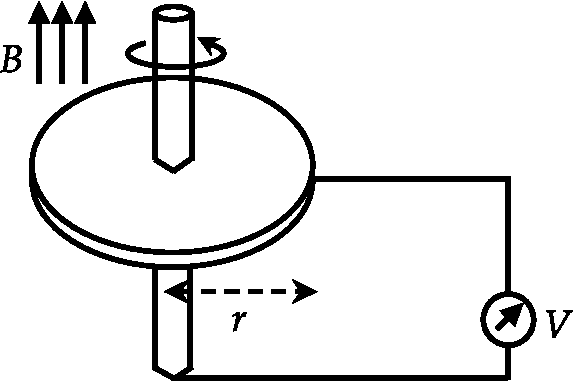
\includegraphics[height=3cm,width=5cm]{diagram-20211011(46)-crop}
	\end{figure}
\end{minipage}
\begin{tasks}(1)
	\task[\textbf{A.}] depends on $\omega, B, r$ and $\rho$
	\task[\textbf{B.}]depends on $\omega, B$ and $r$ but not on $\rho$
	\task[\textbf{C.}]is zero because the flux through the loop is not changing
	\task[\textbf{D.}]is zero because a current the flows in the direction of $B$
\end{tasks}
\begin{answer}
	Force experienced by charge is
	$$
	\vec{F}=q(\vec{v} \times \vec{B}) \text { and } v=r \omega
	$$	
\end{answer}
\begin{minipage}{\textwidth}
	\item A set of $N$ concentric circular loops of wire, each carrying a steady current $I$ in the same direction, is arranged in a plane. The radius of the first loop is $r_{1}=a$ and the radius of the $n^{\text {th }}$ loop is given by $r_{n}=n r_{n-1}$. The magnitude $B$ of the magnetic field at the centre of the circles in the limit $N \rightarrow \infty$, is
	\exyear{NET 2016}
\end{minipage}
\begin{tasks}(2)
	\task[\textbf{A.}] $\mu_{0} I\left(e^{2}-1\right) / 4 \pi a$
	\task[\textbf{B.}]$\mu_{0} I(e-1) / \pi a$
	\task[\textbf{C.}]$\mu_{0} I\left(e^{2}-1\right) / 8 a$
	\task[\textbf{D.}]$\mu_{0} I(e-1) / 2 a$
\end{tasks}
\begin{answer}
	\begin{align*}
	&B=\frac{\mu_{0} I}{2}\left(\frac{1}{r_{1}}+\frac{1}{r_{2}}+\frac{1}{r_{3}}+\ldots \ldots . \frac{1}{r_{n}}\right)\\
	&r_{1}=a \\
	&r_{n}=n r_{n-1} \\
	&r_{1}=r_{0}=a, r_{2}=2 r_{1}=2 a, r_{3}=3 r_{2}=3.2 a \text { and } r_{4}=4 r_{3}=4.3 .2 a \\
	&\Rightarrow B=\frac{\mu_{0} I}{2 a}\left(1+\frac{1}{2}+\frac{1}{3.2}+\frac{1}{4.3 .2}+\ldots \ldots\right) \\
	&B=\frac{\mu_{0} I}{2 a}\left(\sum_{n=1}^{N} \frac{1}{\lfloor n}\right) \\
	&e^{x}=\sum_{n=0}^{\infty} \frac{x^{n}}{\lfloor n} \Rightarrow e=\sum_{n=0}^{\infty} \frac{1}{\lfloor n}=1+\sum_{n=1}^{\infty} \frac{1}{\lfloor n} \Rightarrow \sum_{n=1}^{\infty} \frac{1}{\lfloor n}=e-1 \\
	&\lim _{N \rightarrow \infty}\left(\sum_{n=l}^{N} \frac{1}{n}\right)=e-1 \Rightarrow B=\frac{\mu_{0} I}{2 a}(e-1)
	\end{align*}	
	THe correct option is \textbf{(d)}
\end{answer}
\begin{minipage}{\textwidth}
	\item A constant current $I$ is flowing in a piece of wire that is bent into a loop as shown in the figure.\\
	\begin{figure}[H]
		\centering
		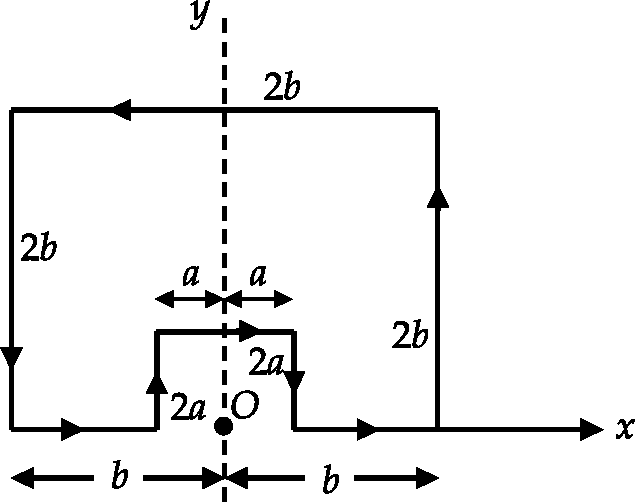
\includegraphics[height=5cm,width=7cm]{diagram-20211011(54)-crop}
	\end{figure}
	$\text { The magnitude of the magnetic field at the point } O \text { is }$
	\exyear{NET 2017}
\end{minipage}
\begin{tasks}(2)
	\task[\textbf{A.}] $\frac{\mu_{0} I}{4 \pi \sqrt{5}} \ln \left(\frac{a}{b}\right)$
	\task[\textbf{B.}]$\frac{\mu_{0} I}{4 \pi \sqrt{5}}\left(\frac{1}{a}-\frac{1}{b}\right)$
	\task[\textbf{C.}]$\frac{\mu_{0} I}{4 \pi \sqrt{5}}\left(\frac{1}{a}\right)$
	\task[\textbf{D.}]$\frac{\mu_{0} I}{4 \pi \sqrt{5}}\left(\frac{1}{b}\right)$
\end{tasks}
\begin{answer}
	\begin{figure}[H]
		\centering
		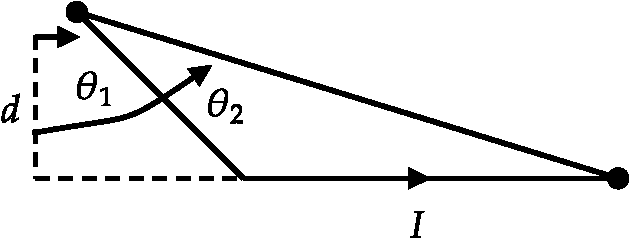
\includegraphics[height=3cm,width=5cm]{diagram-20211011(55)-crop}
	\end{figure}
	\begin{align*}
	\vec{B}&=\frac{\mu_{0} I}{4 \pi d}\left(\sin \theta_{2}-\sin \theta_{1}\right) \hat{\phi}\\
	\intertext{Magnetic field due to left and right segment of 2a}
	B_{2 a}&=\frac{\mu_{0} I}{4 \pi a}\left(\frac{2 a}{\sqrt{5 a}}\right) \otimes\\
	\intertext{Field due to upper segment of $2 a$}
	&=\frac{\mu_{0} I}{4 \pi(2 a)} \times\left(\frac{a}{\sqrt{5} a}+\frac{a}{\sqrt{5} a}\right)\\
	\text{Net field}\\
	B_{2 a}&=2 \times \frac{\mu_{0} I}{4 \pi a} \times \frac{2}{\sqrt{5}}+\frac{\mu_{0} I}{4 \pi a} \times \frac{1}{\sqrt{5}}\\
	B_{2 a}&=\frac{\mu_{0} I}{4 \pi a} \sqrt{5} \otimes(\text { inward })\\
	\text{similarly,} B_{2 b}&=\frac{\mu_{0} I}{4 \pi b} \sqrt{5} \odot \text{(outward)}\\
\text{	Net field}\\
 B&=B_{2 a}-B_{2 b}=\frac{\mu_{0} I}{4 \pi} \sqrt{5}\left(\frac{1}{a}-\frac{1}{b}\right)\\
	\end{align*}
	The correct option is \textbf{(b)}
\end{answer}
\begin{minipage}{\textwidth}
	\item A circular current carrying loop of radius $a$ carries a steady current. A constant electric charge is kept at the centre of the loop. The electric and magnetic fields, $\vec{E}$ and $\vec{B}$ respectively, at a distance $d$ vertically above the centre of the loop satisfy
	\exyear{NET 2017}
\end{minipage}
\begin{tasks}(2)
	\task[\textbf{A.}] $\vec{E} \perp \vec{B}$
	\task[\textbf{B.}] $\vec{E}=0$
	\task[\textbf{C.}]$\vec{\nabla}(\vec{E} \cdot \vec{B})=0$
	\task[\textbf{D.}]$\vec{\nabla} \cdot(\vec{E} \times \vec{B})=0$
\end{tasks}
\begin{answer}
	$\vec{E} \times \vec{B}=0 \Rightarrow \vec{\nabla} \cdot(\vec{E} \times \vec{B})=0$\\
	The correct option is \textbf{(c)}
\end{answer}
\begin{minipage}{\textwidth}
	\item \text { The loop shown in the figure below carries a steady current } I \\
	\begin{figure}[H]
		\centering
		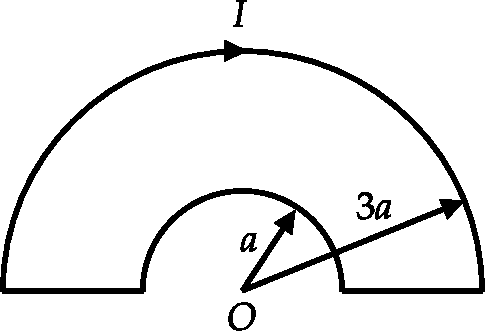
\includegraphics[height=4cm,width=5cm]{diagram-20211011(11)-crop}
	\end{figure}
	$\text { The magnitude of the magnetic field at the point } O \text { is }$
	\exyear{NET 2018}
\end{minipage}
\begin{tasks}(2)
	\task[\textbf{A.}] $\frac{\mu_{0} I}{2 a}$
	\task[\textbf{B.}]$\frac{\mu_{0} I}{6 a}$
	\task[\textbf{C.}]$\frac{\mu_{0} I}{4 a}$
	\task[\textbf{D.}]$\frac{\mu_{0} I}{3 a}$
\end{tasks}
\begin{answer}
	\begin{align*}
	& B_{a}=\frac{1}{2} \frac{\mu_{0} I}{2 a} \odot,\\
	& B_{3 a}=\frac{1}{2} \frac{\mu_{0} I}{2(3 a)} \otimes \\
	&B=B_{a}-B_{3 a}=\frac{\mu_{0} I}{4 a}\left(1-\frac{1}{3}\right)=\frac{\mu_{0} I}{6 a}
	\end{align*}
	THe correct option is \textbf{(b)}	
\end{answer}
\begin{minipage}{\textwidth}
	\item Two current-carrying circular loops, each of radius $R$, are placed perpendicular to each other, as shown in the figure.
	
	The loop in the $x y$ - plane carries a current $I_{0}$ while that in the $x z$-plane carries a current $2 I_{0}$. The resulting magnetic field $\vec{B}$ at the origin is
	\exyear{NET 2018 dec}
	\begin{figure}[H]
		\centering
		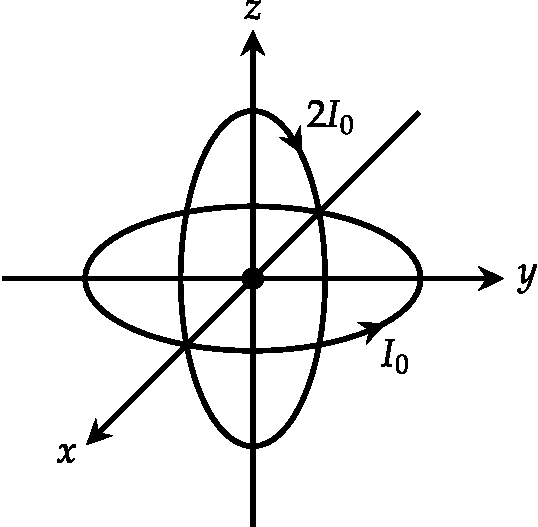
\includegraphics[height=3cm,width=5cm]{diagram-20211011(12)-crop}
	\end{figure}
\end{minipage}
\begin{tasks}(2)
	\task[\textbf{A.}] $\frac{\mu_{0} l_{0}}{2 R}[2 \hat{j}+\hat{k}]$ 
	\task[\textbf{B.}]$\frac{\mu_{0} l_{0}}{2 R}[2 \hat{j}-\hat{k}]$
	\task[\textbf{C.}]$\frac{\mu_{0} l_{0}}{2 R}[-2 \hat{j}+\hat{k}]$
	\task[\textbf{D.}]$\frac{\mu_{0} l_{0}}{2 R}[-2 \hat{j}-\hat{k}]$
\end{tasks}
\begin{answer}
	\begin{align*}
	\intertext{Field due to loop in $x y$ plane is} 
	\vec{B}_{1}&=\frac{\mu_{0} I_{0}}{2 R} \hat{z}\\
	\intertext{Field due to loop in $x z$ plane is}
	\vec{B}_{2}&=\frac{\mu_{0}\left(2 I_{0}\right)}{2 R}(-\hat{y})\\
	\text{Resultant field}\\
	 \vec{B}&=\vec{B}_{1}+\vec{B}_{2}=\frac{\mu_{0} I_{0}}{2 R}(-2 \hat{y}+\hat{z})
	\end{align*}
	The correct option is \textbf{(c)}	
\end{answer}
\end{enumerate}
\newpage
\begin{abox}
	Practice set 2 solutions
	\end{abox}
\begin{enumerate}
	\begin{minipage}{\textwidth}
		\item Two magnetic dipoles of magnitude $m$ each are placed in a plane as shown in figure The energy of interaction is given by
		\exyear{GATE 2010}
		\begin{figure}[H]
			\centering
			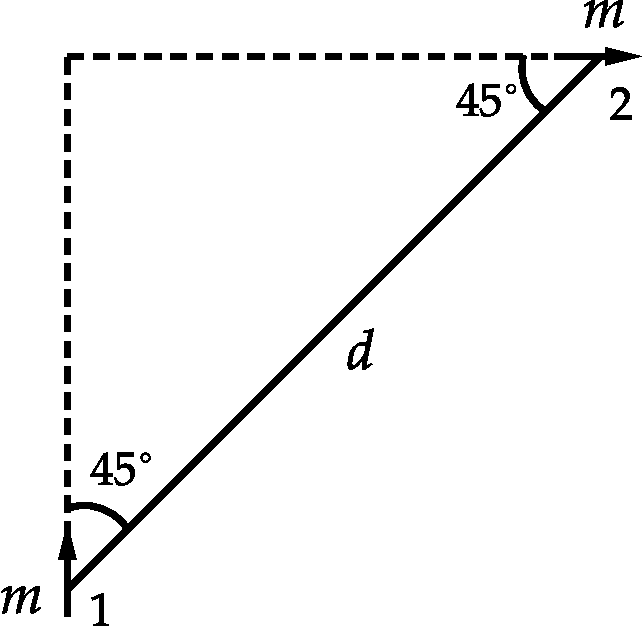
\includegraphics[height=3cm,width=5cm]{diagram-20210817(13)-crop}
			\caption{}
			\label{}
		\end{figure}
	\end{minipage}
	\begin{tasks}(1)
		\task[\textbf{A.}] Zero
		\task[\textbf{B.}]$\frac{\mu_{0} m^{2}}{4 \pi d^{3}}$
		\task[\textbf{C.}]$\frac{3 \mu_{0} m^{2}}{2 \pi d^{3}}$
		\task[\textbf{D.}]$-\frac{3 \mu_{0} m^{2}}{8 \pi d^{3}}$
	\end{tasks}
	\begin{answer}
		\begin{align*}
		U&=\frac{\mu_{0}}{4 \pi r^{3}}\left[\vec{m}_{1} \cdot \bar{m}_{2}-3\left(\vec{m}_{1} \cdot \hat{r}\right)\left(\vec{m}_{2} \cdot \hat{r}\right)\right] \\
		\text { Since } \vec{m}_{1} \perp \vec{m}_{2} &\Rightarrow \vec{m}_{1} \cdot \vec{m}_{2}=0\\
		 U&=\frac{\mu_{0}}{4 \pi d^{3}}\left[-3 \times m \cos 45^{0} \times m \cos 45^{0}\right] \\
		\Rightarrow U&=-\frac{3 \mu_{0} m^{2}}{8 \pi d^{3}}
		\end{align*}	
		The correct option is \textbf{(d)}
	\end{answer}
	\begin{minipage}{\textwidth}
		\item If a force $\vec{F}$ is derivable from a potential function $V(r)$, where $r$ is the distance from the origin of the coordinate system, it follows that
		\exyear{GATE 2011}
	\end{minipage}
	\begin{tasks}(2)
		\task[\textbf{A.}]$\vec{\nabla} \times \vec{F}=0$
		\task[\textbf{B.}]$\vec{\nabla} \cdot \vec{F}=0$
		\task[\textbf{C.}]$\vec{\nabla} V=0$
		\task[\textbf{D.}]$\nabla^{2} V=0$
	\end{tasks}
	\begin{answer}
		The correct option is \textbf{(a)}	
	\end{answer}
	\begin{minipage}{\textwidth}
		\item A uniform surface current is flowing in the positive $y$-direction over an infinite sheet lying in $x-y$ plane. The direction of the magnetic field is
		\exyear{GATE 2011}
	\end{minipage}
	\begin{tasks}(1)
		\task[\textbf{A.}]along $\hat{i}$ for $z>0$ and along $-\hat{i}$ for $z<0$
		\task[\textbf{B.}]along $\hat{k}$ for $z>0$ and along $-\hat{k}$ for $z<0$
		\task[\textbf{C.}]along $-\hat{i}$ for $z>0$ and along $\hat{i}$ for $z<0$
		\task[\textbf{D.}]along $-\hat{k}$ for $z>0$ and along $\hat{k}$ for $z<0$
	\end{tasks}
	\begin{answer}
		The correct option is \textbf{(a)}
	\end{answer}
\begin{minipage}{\textwidth}
	\item A magnetic dipole of dipole moment $\vec{m}$ is placed in a non-uniform magnetic field $\vec{B} .$ If the position vector of the dipole is $\vec{r}$, the torque acting on the dipole about the origin is
	\exyear{GATE 2011}
\end{minipage}
\begin{tasks}(2)
	\task[\textbf{A.}] $\vec{r} \times(\vec{m} \times \vec{B})$
	\task[\textbf{B.}]$\vec{r} \times \vec{\nabla}(\vec{m} \cdot \vec{B})$
	\task[\textbf{C.}]$\vec{m} \times \vec{B}$
	\task[\textbf{D.}]$\vec{m} \times \vec{B}+\vec{r} \times \nabla(\vec{m} \cdot \vec{B})$
\end{tasks}
\begin{answer}
	The correct option is \textbf{(c)}
\end{answer}
	\begin{minipage}{\textwidth}
		\item Which of the following expressions for a vector potential $\vec{A} \underline{\text { DOES NOT }}$ represent a uniform magnetic field of magnitude $B_{0}$ along the $z$-direction?
		\exyear{GATE 2011}
	\end{minipage}
	\begin{tasks}(1)
		\task[\textbf{A.}] $\vec{A}=\left(0, B_{0} x, 0\right)$
		\task[\textbf{B.}]$\vec{A}=\left(-B_{0} y, 0,0\right)$
		\task[\textbf{C.}]$\vec{A}=\left(\frac{B_{0} x}{2}, \frac{B_{0} y}{2}, 0\right)$
		\task[\textbf{D.}] $\vec{A}=\left(-\frac{B_{0} y}{2}, \frac{B_{0} x}{2}, 0\right)$
	\end{tasks}
	\begin{answer}
		$\vec{B} \neq \vec{\nabla} \times \vec{A}$\\
		The correct option is \textbf{(c)}	
	\end{answer}
	
	\begin{minipage}{\textwidth}
		\item In a constant magnetic field of $0.6$ Tesla along the $\mathrm{z}$ direction, find the value of the path integral $\oint \vec{A} \cdot \overrightarrow{d l}$ in the units of (Tesla $m^{2}$ ) on a square loop of side length $(1 / \sqrt{2})$ meters. The normal to the loop makes an angle of $60^{\circ}$ to the z-axis, as shown in the figure.\\
		\begin{figure}[H]
			\centering
			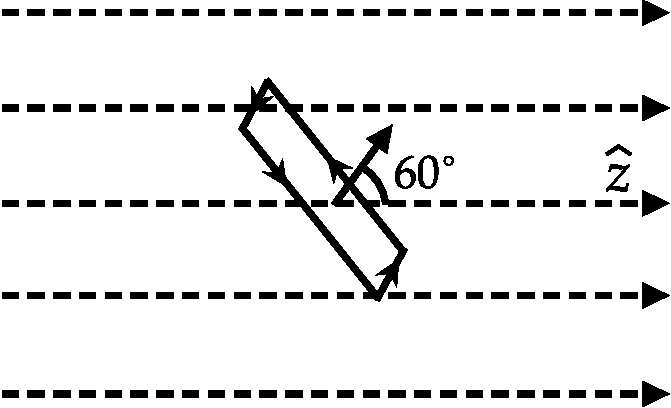
\includegraphics[height=3cm,width=5cm]{diagram-20210817(19)-crop-crop}
		\end{figure}	
		The answer should be up to two decimal places.
		\exyear{GATE}	
	\end{minipage}
	\begin{answer}	
		$$\oint \vec{A} \cdot \overrightarrow{d l}=\int_{S}(\vec{\nabla} \times \vec{A}) d \vec{a}=\int_{S} \vec{B} \cdot d \vec{a}=B A \cos 60^{0}=0.6 \times\left(\frac{1}{\sqrt{2}}\right)^{2} \times \frac{1}{2}=0.15 T . m^{2}$$	
	\end{answer}
	\begin{minipage}{\textwidth}
		\item The value of the magnetic field required to maintain non-relativistic protons of energy $1 \mathrm{MeV}$ in a circular orbit of radius $100 \mathrm{~mm}$ is Tesla
		\exyear{GATE 2014}
	\end{minipage}
	\begin{answer}
	\begin{align*}	
	E&=\frac{q^{2} B^{2} R^{2}}{2 m_{p}} \Rightarrow 1.6 \times 10^{-13}=\frac{\left(1.6 \times 10^{-19}\right)^{2} B^{2}(0.1)^{2}}{2\left(1.67 \times 10^{-27}\right)}\\
	\Rightarrow B^{2}&=\frac{1.6 \times 10^{-13} \times 2\left(1.67 \times 10^{-27}\right)}{\left(1.6 \times 10^{-19}\right)^{2}(0.1)^{2}} \\
	\Rightarrow B^{2}&=\frac{10^{-13} \times 2\left(1.67 \times 10^{-27}\right)}{\left(1.6 \times 10^{-38}\right)(0.01)}=\frac{3.34 \times 10^{-40}}{1.6 \times 10^{-40}}=2.08\\
	\Rightarrow B&=\sqrt{2.08} \text { Tesla }=1.44 \text { Tesla }
	\end{align*}	
	\end{answer}
	\begin{minipage}{\textwidth}
		\item Given that the magnetic flux through the closed loop $P Q R S P$ is $\phi$. If $\int_{P}^{R} \vec{A} \cdot \vec{d} l=\phi_{1}$ along $P Q R$, the value of $\int^{R} \vec{A} \cdot \vec{d} l$ along $P S R$ is
		\exyear{GATE 2015}
		\begin{figure}[H]
			\centering
			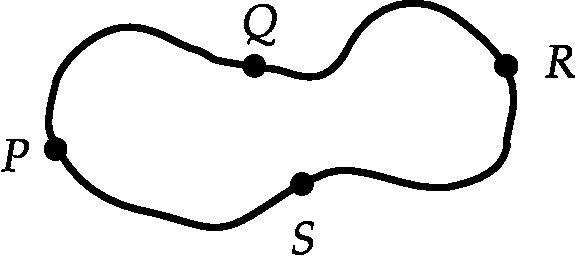
\includegraphics[height=3cm,width=5cm]{diagram-20210818(2)-crop}
		\end{figure}
	\end{minipage}
	\begin{tasks}(2)
		\task[\textbf{A.}](a) $\phi-\phi_{1}$
		\task[\textbf{B.}] $\phi_{1}-\phi$
		\task[\textbf{C.}]$-\phi_{1}$
		\task[\textbf{D.}] $\phi_{1}$
	\end{tasks}
	\begin{answer}
		$$\phi=\int_{s} \vec{B} \cdot d \vec{a}=\oint \vec{A} \cdot d \vec{l}=\int_{P}^{R} \vec{A} \cdot d \vec{l}+\int_{R}^{P} \vec{A} \cdot d \vec{l} \Rightarrow \phi=\phi_{1}-\int_{P}^{R} \vec{A} \cdot d \vec{l} \Rightarrow \int_{P}^{R} \vec{A} \cdot d \vec{l}=\phi_{1}-\phi$$
		The correct option is \textbf{(b)}	
	\end{answer}
	\begin{minipage}{\textwidth}
		\item Which of the following magnetic vector potentials gives rise to a uniform magnetic field $B_{0} \hat{k} ?$
		\exyear{GATE 2016}
	\end{minipage}
	\begin{tasks}(2)
		\task[\textbf{A.}] $B_{0} z \hat{k}$
		\task[\textbf{B.}]$-B_{0} x \hat{j}$
		\task[\textbf{C.}]$\frac{B_{0}}{2}(-y \hat{i}+x \hat{j})$
		\task[\textbf{D.}]$\frac{B_{0}}{2}(y \hat{i}+x \hat{j})$
	\end{tasks}
	\begin{answer}
		(a) $\vec{\nabla} \times \vec{A}=0$\\
		(b) $\vec{\nabla} \times \vec{A}=-B_{0} \hat{k}$\\
		(c) $\vec{\nabla} \times \vec{A}=B_{0} \hat{k}$\\
		(d) $\vec{\nabla} \times \vec{A}=0$\\
		The correct option is \textbf{(c)}
	\end{answer}
	\begin{minipage}{\textwidth}
		\item The magnitude of the magnetic dipole moment associated with a square shaped loop carrying a steady current $I$ is $m$. If this loop is changed to a circular shape with the same current $I$ passing through it, the magnetic dipole moment becomes $\frac{p m}{\pi} .$ The value of $p$ is
		\exyear{GATE 2016}
	\end{minipage}
	\begin{answer}
		Magnetic dipole moment associated with a square shaped loop (let side is $a$ ) carrying a steady current $I$ is $m=I a^{2}$.
		
		Magnetic dipole moment associated with a circular shaped loop (let radius is $r$ ) carrying a steady current $I$ is $m^{\prime}=I \pi r^{2}$.
		Here $4 a=2 \pi r \Rightarrow r=\frac{2 a}{\pi} \Rightarrow m^{\prime}=I \pi r^{2}=I \pi\left(\frac{2 a}{\pi}\right)^{2}=\frac{4 I a^{2}}{\pi}=\frac{4 m}{\pi}$	
	\end{answer}
	\begin{minipage}{\textwidth}
		\item An infinite solenoid carries a time varying current $I(t)=A t^{2}$, with $A \neq 0 .$ The axis of the solenoid is along the $\hat{z}$ direction. $\hat{r}$ and $\hat{\theta}$ are the usual radial and polar directions in cylindrical polar coordinates. $\vec{B}=B_{r} \hat{r}+B_{\theta} \hat{\theta}+B_{z} \hat{z}$ is the magnetic field at a point outside the solenoid. Which one of the following statements is true?
		\exyear{GATE 2017}
	\end{minipage}
	\begin{tasks}(2)
		\task[\textbf{A.}] $B_{r}=0, B_{\theta}=0, B_{z}=0$
		\task[\textbf{B.}]$B_{r} \neq 0, B_{\theta} \neq 0, B_{z}=0$
		\task[\textbf{C.}] $B_{r} \neq 0, B_{\theta} \neq 0, B_{z} \neq 0$
		\task[\textbf{D.}] $B_{r}=0, B_{\theta}=0, B_{z} \neq 0$
	\end{tasks}
	\begin{answer}
		The correct option is \textbf{(d)}	
	\end{answer}
	\begin{minipage}{\textwidth}
		\item An infinitely long straight wire is carrying a steady current $I$. The ratio of magnetic energy density at distance $r_{1}$ to that at $r_{2}\left(=2 r_{1}\right)$ from the wire is
		\exyear{GATE 2018}
	\end{minipage}
	\begin{answer}
		$$ u_{B}=\frac{B^{2}}{2 \mu_{0}} \propto \frac{1}{r^{2}} \Rightarrow \frac{u_{B 1}}{u_{B 2}}=\frac{r_{2}^{2}}{r_{1}^{2}}=\frac{\left(2 r_{1}\right)}{r_{1}^{2}}=4$$	
	\end{answer}
	\begin{minipage}{\textwidth}
		\item A constant and uniform magnetic field $\vec{B}=B_{0} \hat{k}$ pervades all space. Which one of the following is the correct choice for the vector potential in Coulomb gauge?
		\exyear{GATE 2018}
	\end{minipage}
	\begin{tasks}(1)
		\task[\textbf{A.}] $-B_{0}(x+y) \hat{i}$
		\task[\textbf{B.}]$B_{0}(x+y) \hat{j}$
		\task[\textbf{C.}] $B_{0} x \hat{j}$
		\task[\textbf{D.}]$-\frac{1}{2} B_{0}(x \hat{i}-y \hat{j})$
	\end{tasks}
	\begin{answer}
		Check option (c),
		$$
		\vec{\nabla} \cdot \vec{A}=0, \vec{B}=\vec{\nabla} \times \vec{A}=B_{0} \hat{k}
		$$
		The correct option is \textbf{(c)}
	\end{answer}
	\begin{minipage}{\textwidth}
		\item  A solid cylinder of radius $R$ has total charge $Q$ distributed uniformly over its volume. It is rotating about its axis with angular speed $\omega$. The magnitude of the total magnetic moment of the cylinder is
		\exyear{GATE 2019}
	\end{minipage}
	\begin{tasks}(2)
		\task[\textbf{A.}](a) $Q R^{2} \omega$
		\task[\textbf{B.}]$\frac{1}{2} Q R^{2} \omega$
		\task[\textbf{C.}]$\frac{1}{4} Q R^{2} \omega$
		\task[\textbf{D.}]$\frac{1}{8} Q R^{2} \omega$
	\end{tasks}
	\begin{answer}
\begin{align*}
	\intertext{	Magnetic moment due to disc} 
\mu&=\frac{\pi \sigma \omega R^{4}}{4}\\
\text{	Due to cylinder}\\
 d \mu&=\frac{\pi \omega R^{4}}{4}(\rho d z) \quad(\sigma \rightarrow \rho d z)\\
\mu&=\frac{\pi \omega R^{4}}{4} \int_{0}^{L} \frac{Q}{\pi R^{2} L} d z=\frac{Q \omega R^{4}}{4}	
\end{align*}
	\end{answer}
	\begin{minipage}{\textwidth}
		\item An infinitely long wire parallel to the $x$-axis is kept at $z=d$ and carries a current $I$ in the positive $x$ direction above a superconductor filling the region $z \leq 0$ (see figure). The magnetic field $\vec{B}$ inside the superconductor is zero so that the field just outside the superconductor is parallel to its surface. The magnetic field due to this configuration at a point $(x, y, z>0)$ is
		\exyear{GATE 2019}
		\begin{figure}[H]
			\centering
			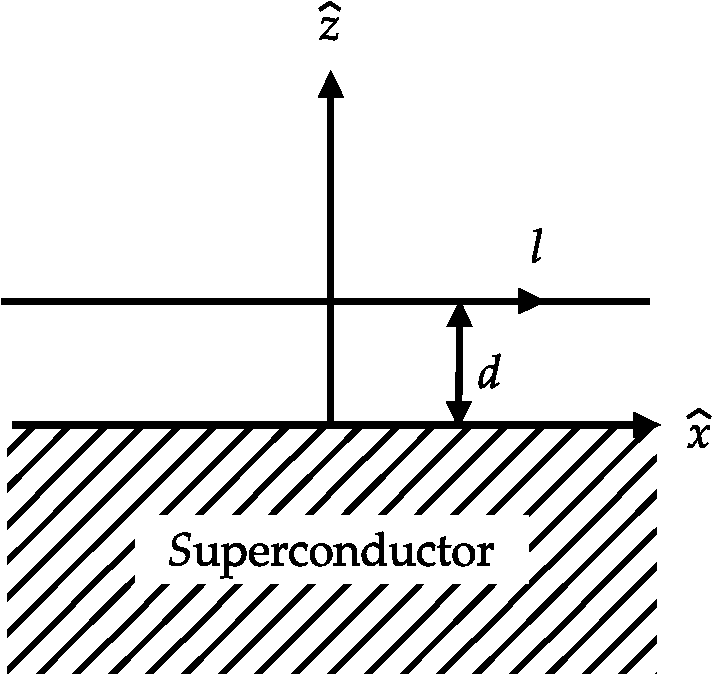
\includegraphics[height=5cm,width=5cm]{diagram-20210818(14)-crop-crop}
			\caption{}
			\label{}
		\end{figure}
	\end{minipage}
	\begin{tasks}(1)
		\task[\textbf{A.}]$\left(\frac{\mu_{0} I}{2 \pi}\right) \frac{-(z-d) \hat{j}+y \hat{k}}{\left[y^{2}+(z-d)^{2}\right]}$
		\task[\textbf{B.}]$\left(\frac{\mu_{0} I}{2 \pi}\right)\left[\frac{-(z-d) \hat{j}+y \hat{k}}{y^{2}+(z-d)^{2}}+\frac{(z+d) \hat{j}-y \hat{k}}{y^{2}+(z+d)^{2}}\right]$
		\task[\textbf{C.}]$\text { (c) }\left(\frac{\mu_{0} I}{2 \pi}\right)\left[\frac{-(z-d) \hat{j}+y \hat{k}}{y^{2}+(z-d)^{2}}-\frac{(z+d) \hat{j}-y \hat{k}}{y^{2}+(z+d)^{2}}\right]$
		\task[\textbf{D.}]$\text { (d) }\left(\frac{\mu_{0} I}{2 \pi}\right)\left[\frac{y \hat{j}+(z-d) \hat{k}}{y^{2}+(z-d)^{2}}+\frac{y \hat{j}-(z+d) \hat{k}}{y^{2}+(z+d)^{2}}\right]$
	\end{tasks}
	\begin{answer}
		$\text { Verify that } \vec{B}=0, \text { when } d=0$\\
		The correct option is \textbf{(b)}	
	\end{answer}
	\begin{minipage}{\textwidth}
		\item The vector potential inside a long solenoid with $n$ turns per unit length and carrying current $I$, written in cylindrical coordinates is $\vec{A}(s, \phi, z)=\frac{\mu_{0} n I}{2} s \hat{\phi}$. If the term $\frac{\mu_{0} n I}{2} s(\alpha \cos \phi \hat{\phi}+\beta \sin \phi \hat{s})$, where $\alpha \neq 0, \beta \neq 0$ is added to $\vec{A}(S, \phi, z)$, the magnetic field remains the same if
		\exyear{GATE 2019}
	\end{minipage}
	\begin{tasks}(2)
		\task[\textbf{A.}]$\alpha=\beta$
		\task[\textbf{B.}]$\alpha=-\beta$
		\task[\textbf{C.}]$\alpha=2 \beta$
		\task[\textbf{D.}]$\alpha=\frac{\beta}{2}$
	\end{tasks}
	\begin{answer}
		\begin{align*}
		&\text { Solution: } \vec{B}=\vec{\nabla} \times \vec{A}=\frac{1}{r}\left|\begin{array}{ccc}
		\hat{r} & r \hat{\phi} & \hat{z} \\
		\frac{\partial}{\partial r} & \frac{\partial}{\partial \phi} & \frac{\partial}{\partial z} \\
		A_{r} & r A_{\phi} & 0
		\end{array}\right|=\mu_{0} n I \hat{z} \\
		&\vec{B}^{\prime}=\vec{\nabla} \times \vec{A}^{\prime}=\frac{1}{r}\left|\begin{array}{ccc}
		\hat{r} & r \hat{\phi} & \hat{z} \\
		\frac{\partial}{\partial r} & \frac{\partial}{\partial \phi} & \frac{\partial}{\partial z} \\
		A_{r} & r A_{\phi} & 0
		\end{array}\right|=\mu_{0} n I\left[(\alpha \cos \phi+1)-\frac{\beta \cos \phi}{2}\right] \hat{z} \\
		&\text { Equate } \vec{B}^{\prime}=\vec{B} \Rightarrow\left[(\alpha \cos \phi+1)-\frac{\beta \cos \phi}{2}\right]=\mu_{0} n I \\
		&\Rightarrow \alpha \cos \phi=\frac{\beta}{2} \cos \phi \Rightarrow \alpha=\frac{\beta}{2}
		\end{align*}
		The correct option is \textbf{(d)}	
	\end{answer}
	\begin{minipage}{\textwidth}
		\item A magnetic field $\vec{B}=B_{0}(\hat{i}+2 \hat{j}-4 \hat{k})$ exists at point. If a test charge moving with a velocity, $\vec{v}=v_{0}(3 \hat{i}-\hat{j}+2 \hat{k})$ experiences no force at a certain point, the electric field at that point in SI units is
		\exyear{JEST 2012}
	\end{minipage}
	\begin{tasks}(2)
		\task[\textbf{A.}] $\vec{E}=-v_{0} B_{0}(3 \hat{i}-2 \hat{j}-4 \hat{k})$
		\task[\textbf{B.}]$\vec{E}=-v_{0} B_{0}(\hat{i}+\hat{j}+7 \hat{k})$
		\task[\textbf{C.}]$\vec{E}=v_{0} B_{0}(14 \hat{j}+7 \hat{k})$
		\task[\textbf{D.}]$\vec{E}=-v_{0} B_{0}(14 \hat{j}+7 \hat{k})$
	\end{tasks}
	\begin{answer}
		 \begin{align*}
		\vec{F} &=q[\vec{E}+\vec{v} \times \vec{B}]=0 \Rightarrow \vec{E}=-(\vec{v} \times \vec{B}) \\
		\Rightarrow \vec{E} &=-v_{0} B_{0}\{(4-4) \hat{i}+(2+12) \hat{j}+(6+1) \hat{k}\}\\
		&=-v_{0} B_{0}(14 \hat{j}+7 \hat{k})
		\end{align*}
	\end{answer}
	\begin{minipage}{\textwidth}
		\item A small magnet is dropped down a long vertical copper tube in a uniform gravitational field. After a long time, the magnet
		\exyear{JEST 2012}
	\end{minipage}
	\begin{tasks}(2)
		\task[\textbf{A.}] attains a constant velocity
		\task[\textbf{B.}] moves with a constant acceleration
		\task[\textbf{C.}] moves with a constant deceleration
		\task[\textbf{D.}]executes simple harmonic motion
	\end{tasks}
	\begin{answer}
		The correct option is \textbf{(a)}
	\end{answer}
	\begin{minipage}{\textwidth}
		\item A thin uniform ring carrying charge $Q$ and mass $M$ rotates about its axis. What is the gyromagnetic ratio (defined as ratio of magnetic dipole moment to the angular momentum) of this ring?
		\exyear{JEST 2013}
	\end{minipage}
	\begin{tasks}(2)
		\task[\textbf{A.}] $\frac{Q}{2 \pi M}$
		\task[\textbf{B.}]$\frac{Q}{M}$
		\task[\textbf{C.}]$\frac{Q}{2 M}$
		\task[\textbf{D.}]$\frac{Q}{\pi M}$
	\end{tasks}
	\begin{answer}
		Magnetic dipole moment $M^{\prime}=I A=\frac{Q}{T} \pi r^{2} \Rightarrow \frac{Q}{2 \pi T} \times 2 \pi \times \pi r^{2}=\frac{Q \omega r^{2}}{2}$\\
		Angular momentum $J=M r^{2} \omega \Rightarrow \frac{M^{\prime}}{J}=\frac{Q}{2 M}$	
	\end{answer}
	\begin{minipage}{\textwidth}
		\item The electric and magnetic field caused by an accelerated charged particle are found to scale as $E \propto r^{-n}$ and $B \propto r^{-m}$ at large distances. What are the value of $n$ and $m$ ?
		\exyear{JEST 2013}
	\end{minipage}
	\begin{tasks}(2)
		\task[\textbf{A.}] $n=1, m=2$
		\task[\textbf{B.}] $n=2, m=1$
		\task[\textbf{C.}]$n=1, m=1$
		\task[\textbf{D.}]$n=2, m=2$
	\end{tasks}
	\begin{answer}
	\begin{align*}
		\intertext{For large distance}
	F&=\frac{q a \sin \theta}{r}\\
	, B&=\frac{q a \sin \theta}{r}\\
	\Rightarrow E &\propto \frac{1}{r},\\
	B &\propto \frac{1}{r} \\
	\text{So} \quad m&=n=1
	\end{align*}
		The correct option is \textbf{(c)}	
	\end{answer}
	\begin{minipage}{\textwidth}
		\item A system of two circular co-axial coils carrying equal currents $I$ along same direction having equal radius $R$ and separated by a distance $R$ (as shown in the figure below). The magnitude of magnetic field at the midpoint $P$ is given by
		\exyear{JEST 2014}
		\begin{figure}[H]
			\centering
			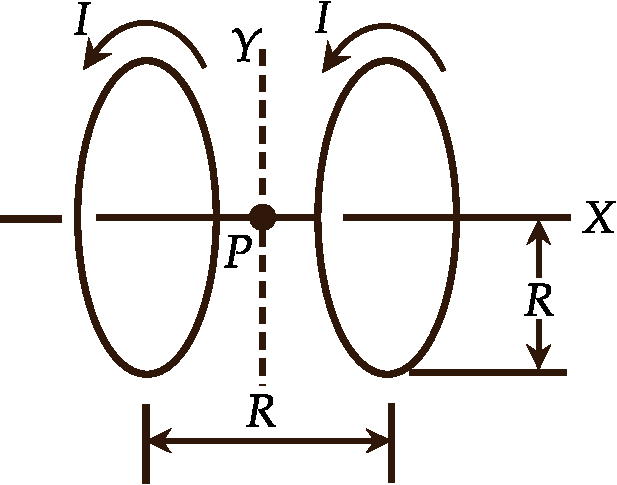
\includegraphics[height=3cm,width=5cm]{diagram-20210809(7)-crop}
			\caption{}
			\label{}
		\end{figure}
	\end{minipage}
	\begin{tasks}(2)
		\task[\textbf{A.}](a) $\frac{\mu_{0} I}{2 \sqrt{2} R}$
		\task[\textbf{B.}]$\frac{4 \mu_{0} I}{5 \sqrt{5} R}$
		\task[\textbf{C.}]$\frac{8 \mu_{0} I}{5 \sqrt{5} R}$
		\task[\textbf{D.}] 0
	\end{tasks}
	\begin{answer}
		\begin{align*}
		\because B&=\frac{\mu_{0} I R^{2}}{2\left(R^{2}+d^{2}\right)^{\frac{3}{2}}}\\ B_{1}&=\frac{\mu_{0} I R^{2}}{2\left(R^{2}+\frac{R^{2}}{4}\right)^{\frac{3}{2}}}\\
		B_{2}&=\frac{\mu_{0} I R^{2}}{2\left(R^{2}+\frac{R^{2}}{4}\right)^{\frac{3}{2}}} \because d=\frac{R}{2} \\
		B&=B_{1}+B_{2}\\
		&=\frac{\mu_{0} I \times 2}{2 R\left(\frac{5}{4}\right)^{\frac{3}{2}}}\\
		B&=\frac{\mu_{0} I 4^{\frac{3}{2}}}{R \quad 5^{\frac{3}{2}}}=\frac{8 \mu_{0} I}{5 \sqrt{5} R}
		\end{align*}
		The correct option is \textbf{(c)}	
	\end{answer}
	\begin{minipage}{\textwidth}
		\item A charged particle is released at time $t=0$, from the origin in the presence of uniform static electric and magnetic fields given by $E=E_{0} \hat{y}$ and $B=B_{0} \hat{z}$ respectively. Which of the following statements is true for $t>0$ ?
		\exyear{JEST 2015}
	\end{minipage}
	\begin{tasks}(2)
		\task[\textbf{A.}] The particle moves along the $x$-axis.
		\task[\textbf{B.}]The particle moves in a circular orbit.
		\task[\textbf{C.}]The particle moves in the $(x, y)$ plane.
		\task[\textbf{D.}] Particle moves in the $(y, z)$ plane
	\end{tasks}
	\begin{answer}
		In a cycloid charged particle will be always confined in a plane perpendicular to B.\\
		The correct option is \textbf{(c)}
	\end{answer}
	\begin{minipage}{\textwidth}
		\item The strength of magnetic field at the center of a regular hexagon with sides of length $a$ carrying a steady current $I$ is:
		\exyear{JEST 2016}
	\end{minipage}
	\begin{tasks}(2)
		\task[\textbf{A.}] $\frac{\mu_{0} I}{\sqrt{3} \pi a}$ 
		\task[\textbf{B.}]$\frac{\sqrt{6} \mu_{0} I}{\pi a}$
		\task[\textbf{C.}]$\frac{3 \mu_{0} I}{\pi a}$
		\task[\textbf{D.}]$\frac{\sqrt{3} \mu_{0} I}{\pi a}$
	\end{tasks}
	\begin{answer}
		\begin{figure}[H]
			\centering
			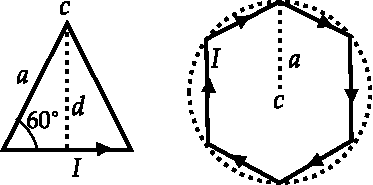
\includegraphics[height=3cm,width=6cm]{jest 3-crop}
		\end{figure}
		\begin{align*}
		d&=a \cos 30^{\circ}=\frac{\sqrt{3}}{2} a \\
		\because B&=\frac{\mu_{0} I}{4 \pi d}\left(\sin \theta_{2}-\sin \theta_{1}\right) \\
		\Rightarrow B_{1}&=\frac{\mu_{0} I}{4 \pi d} 2 \sin 30^{\circ}=\frac{\mu_{0} I}{4 \pi \frac{\sqrt{3}}{2} a} 2 \sin 30^{\circ}=\frac{\mu_{0} I}{2 \sqrt{3} \pi a} \\
		\Rightarrow B&=6 B_{1}=6 \times \frac{\mu_{0} I}{2 \sqrt{3} \pi a}=\frac{3 \mu_{0} I}{\sqrt{3} \pi a}=\frac{\sqrt{3} \mu_{0} I}{\pi a}
		\end{align*}
	\end{answer}
	\begin{minipage}{\textwidth}
		\item A wire with uniform line charge density $\lambda$ per unit length carries a current $I$ as shown in the figure. Take the permittivity and permeability of the medium to be $\varepsilon_{0}=\mu_{0}=1 . \mathrm{A}$ particle of charge $q$ is at a distance $r$ and is travelling along a trajectory parallel to the wire. What is the speed of the charge?
		\exyear{JEST 2019}
		\begin{figure}[H]
			\centering
			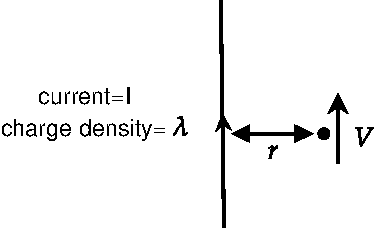
\includegraphics[height=4cm,width=6cm]{jest-crop}
		\end{figure}
	\end{minipage}
	\begin{tasks}(2)
		\task[\textbf{A.}] $\frac{\lambda}{I}$ 
		\task[\textbf{B.}]$\frac{\lambda}{2 I}$
		\task[\textbf{C.}]$\frac{\lambda}{3 I}$
		\task[\textbf{D.}]$\frac{4 \lambda}{I}$
	\end{tasks}
	\begin{answer}
		\begin{figure}[H]
			\centering
			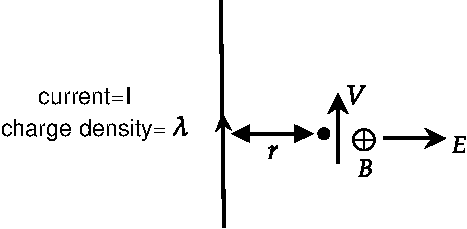
\includegraphics[height=3cm,width=5cm]{jest2-crop(1)}
		\end{figure}
	\begin{align*}
		E&=\frac{\lambda}{2 \pi \varepsilon_{0} r} \text { and } B=\frac{\mu_{0} I}{2 \pi r}\\
	\intertext{Net force on  $q$ is zero i.e.}
	\vec{F}&=0\\
	\Rightarrow q[\vec{E}+(\vec{v} \times \vec{B})]&=0\\
	E&=v B \Rightarrow \frac{\lambda}{2 \pi \varepsilon_{0} r}=v \frac{\mu_{0} I}{2 \pi r} \Rightarrow v=\frac{\lambda}{I} \quad \because \varepsilon_{0}=\mu_{0}=1
	\end{align*}
The correct option is \textbf{(a)}	
	\end{answer}
\end{enumerate}